\documentclass[12pt,a4paper,oneside]{article}
%\documentclass[12pt,a4paper,oneside,twocolumn]{article}
\usepackage{pagestyle}
\usepackage{codestyle}

% Report hand-in date
\DTMsavedate{date}{2024-03-29}

\title{
    \Huge{Machine Learning} \\ \LARGE 
    Nature's Quest: Deep Learning Exploration of Global Plant Traits from Images and Geodata
}
\author{
Kai E. Niermann \and
Dávid Miklo \and 
Trix Taicet \and
Red Kaláb \and
Conner Dassen
}
\date{\DTMusedate{date}}
\begin{document}
\maketitle

% \lstinputlisting[firstline=10, lastline=13]{code/sample_script.py}

\begin{abstract}
    Global warming and climate change have created concerns about the adaptation of plant species to constantly evolving environmental conditions. Monitoring and analyzing plant traits provides crucial insights into ecosystem responses to such changes. Convolutional Neural Networks (CNNs) offer a promising approach to predicting plant traits based on images and related geological and satellite data. This paper explores the effectiveness of CNNs predicting relevant plant traits trained on images alone versus those trained on images combined with ancillary geodata. Our results indicate that while models trained on images and geodata converge faster, they do not necessarily outperform models trained on images alone. Further investigation into hyperparameters, model architectures, and data modifications is warranted to enhance these models' predictive capabilities and understand the relationship between plant traits and environmental factors.    
\end{abstract}

\section{Introduction}
% primary paragraph 
Global warming and, more broadly, climate change have become a major concern for the world as its effects are becoming increasingly apparent \cite{WANG2023100237}. Changing weather patterns, especially towards more extreme conditions, are causing plants to adapt to new environments \cite{GRAY201664}. One method of measuring said adaptation is to look at the traits, that is, properties of a plant that describe how it functions and interacts with the environment. These traits include but are not limited to the plant height, leaf area, dry mass, and leaf nitrogen content, amongst various others. Monitoring these traits allows us to gain vital insights into how climate change impacts different ecosystems. While somewhat simple manual measurement techniques exist, they are not feasible at scale. This is where Convolutional Neural Networks (CNN) come in.  

\smallskip
Through the work demonstrated by Schiller et al. \cite{schiller2021deep}, we know that CNNs can be used to predict plant traits from images. The images used to train this network came from \textit{citizen science photographs} and are taken by citizens of plants worldwide using AI plant identification apps (e.g., iNaturalist, Pl@ntNet). Citizen science photographs also come with location metadata, which can be used to extract ancillary geodata such as precipitation, temperature, and soil type. This geodata can optionally be combined with the images to create a CNN, which can potentially learn to extract features from images in conjunction with geodata to predict plant traits.

\smallskip
For our method, we wanted to compare the accuracy of a CNN trained on images alone and using a pre-trained backbone (e.g., ResNet, EfficientNet, etc.) to a CNN trained on images and geodata. We hypothesize that the CNN trained on images and geodata will outperform the CNN trained on images alone. With our results, we hope to provide a better understanding of the key factors needed to predict plant traits.

% secondary paragraph
% \section{Literature review}

\section{Method}

\subsection{Data processing}

Integral to any machine learning model is the data used to train, validate, and ultimately test it. The data used consisted of three main components: ancillary geodata from various sources, the main task trait means and auxiliary task standard deviations, and the training images of the plants.

\smallskip 
Upon visual inspection, one of the first issues we spotted was a considerable chunk (29.53\%) of data missing for the auxiliary task standard deviations. Previous work on the same Kaggle showed us that the auxiliary data was a useful inclusion. We can also validate these reports with previous work applying auxiliary tasks in CNNs, such as the work of Lukas Libel and Marco Kroener, which found that the inclusion of an auxiliary task with minor relevance to the main task did indeed boost performance \cite{lukaslibel}. Chen et al. \cite{pmlr-v80-chen18a} demonstrated that for very similar or mostly similar auxiliary tasks, the contribution is generally a positive one. Based on this, we decided to use a simple k-nearest neighbor (kNN) imputation strategy, which has generally proven effective \cite{joel2024performance}. The rest of the data had all values present.

\smallskip
The geodata was another point of consideration in the data pre-processing phase. Looking at the individual columns, we noticed that the instances had features that encoded similar information and, thus, were likely redundant during the training process. Since we are working with a very high dimensional feature space to get some visual verification of this claim, we plotted a correlation heatmap for the three biggest groups of the geodata, namely the datasets: SOIL, MODIS, and VOD.

\begin{figure}[!h]
    \centering
    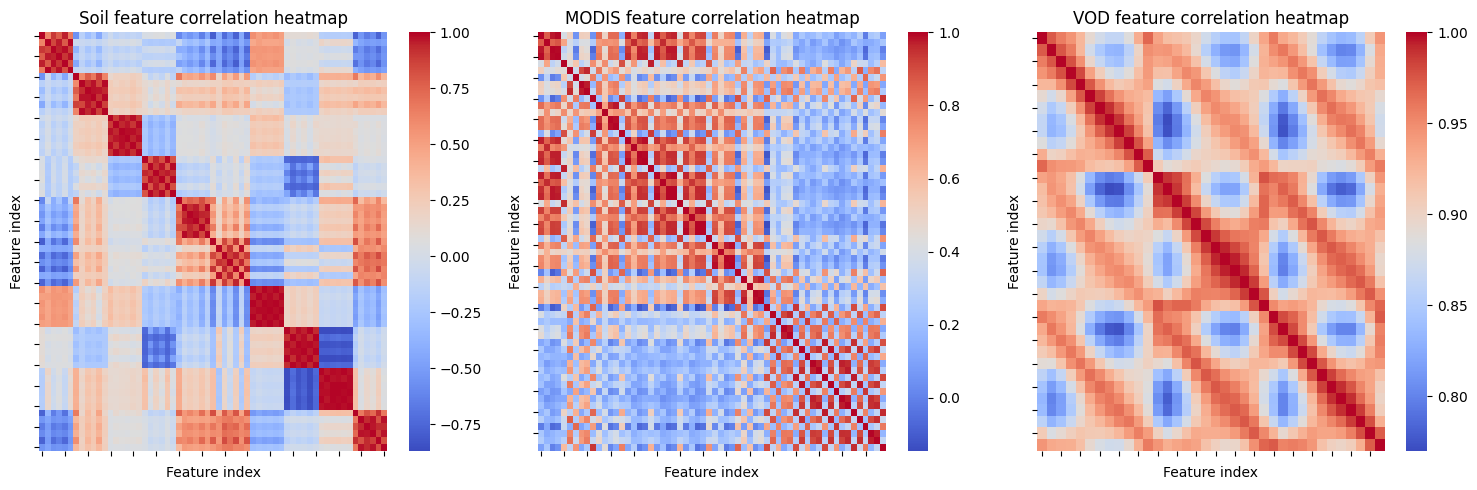
\includegraphics[width=0.9\textwidth]{assets/corr_hm.png}
    \caption{Correlation heatmap of the 3 biggest groups of geodata}
\end{figure}

Since these datasets can be broken down into groups of features that generally talk about a similar topic (e.g., precipitation metrics, temperature metrics, etc.), we can see that the correlation within these groups is relatively high. Even though previous work \cite{DBLP:journals/corr/abs-2007-00062} has demonstrated the viability of neural network models to learn from high dimensional data, removing redundant features has in numerous instances been shown to improve model performance \cite{chen2022survey}. With this in mind, we decided to apply a Principal Component Analysis (PCA) to the geodata to reduce the dimensionality of the data. We specified that the number of principal components should be such that 95\% of the variance is explained.  

\subsection{Data preparation}

% talk about the augmentation 
Our training and test image instance - consisting of science citizen photographs - was taken by a wide variety of people under a wide variety of conditions. This means the images are of varying quality, resolution, and orientation. We can see this just by taking a random sample of 5 images.
\begin{figure}[!h]
    \centering
    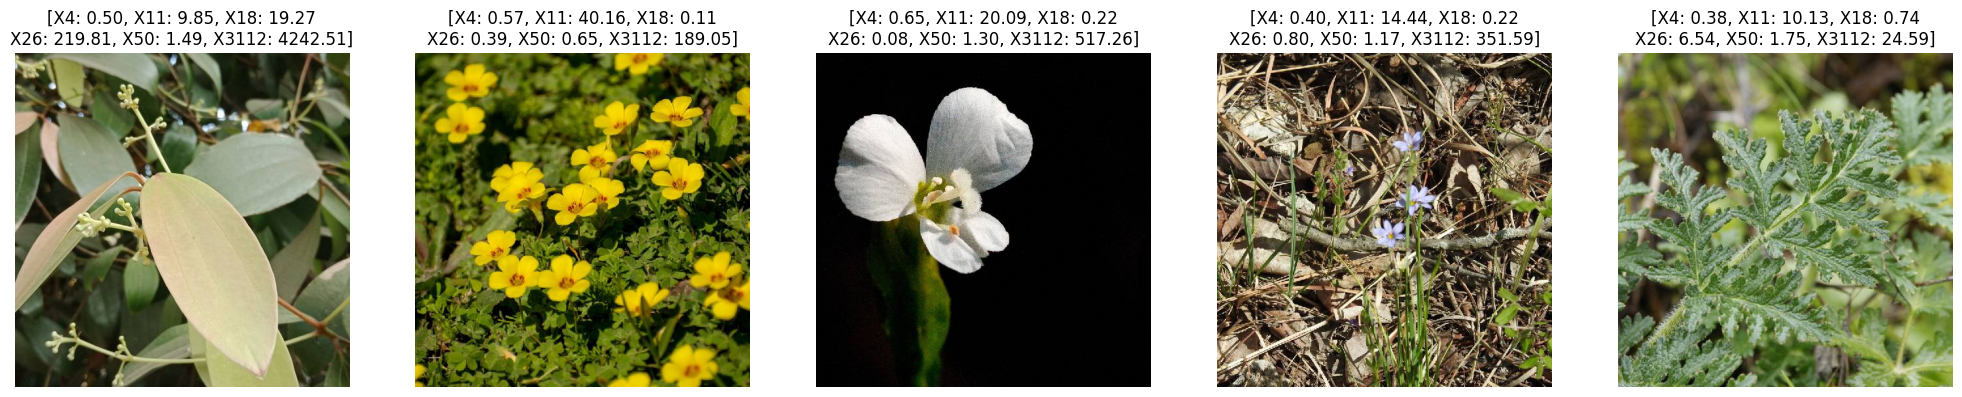
\includegraphics[width=0.9\textwidth]{assets/before_aug_img.png}
    \caption{Random sample of 5 images before augmentation annotated with their target trait labels}
\end{figure}

To prevent our model from fitting to noise in the data as a byproduct of how images were taken, we applied different Keras preprocessing layers to batches concurrently. A key benefit would be that the model can generalize better to unseen data by learning potentially more meaningful features. While this approach of applying augmentations in the preprocessing stage is less flexible than having filters integrated into the model, it does reduce model complexity, though at the cost of potentially losing some ability to learn more complex features by being able to adjust the filters dynamically. After sampling again, we can look at the results of our augmentations. 

\begin{figure}[!h]
    \centering
    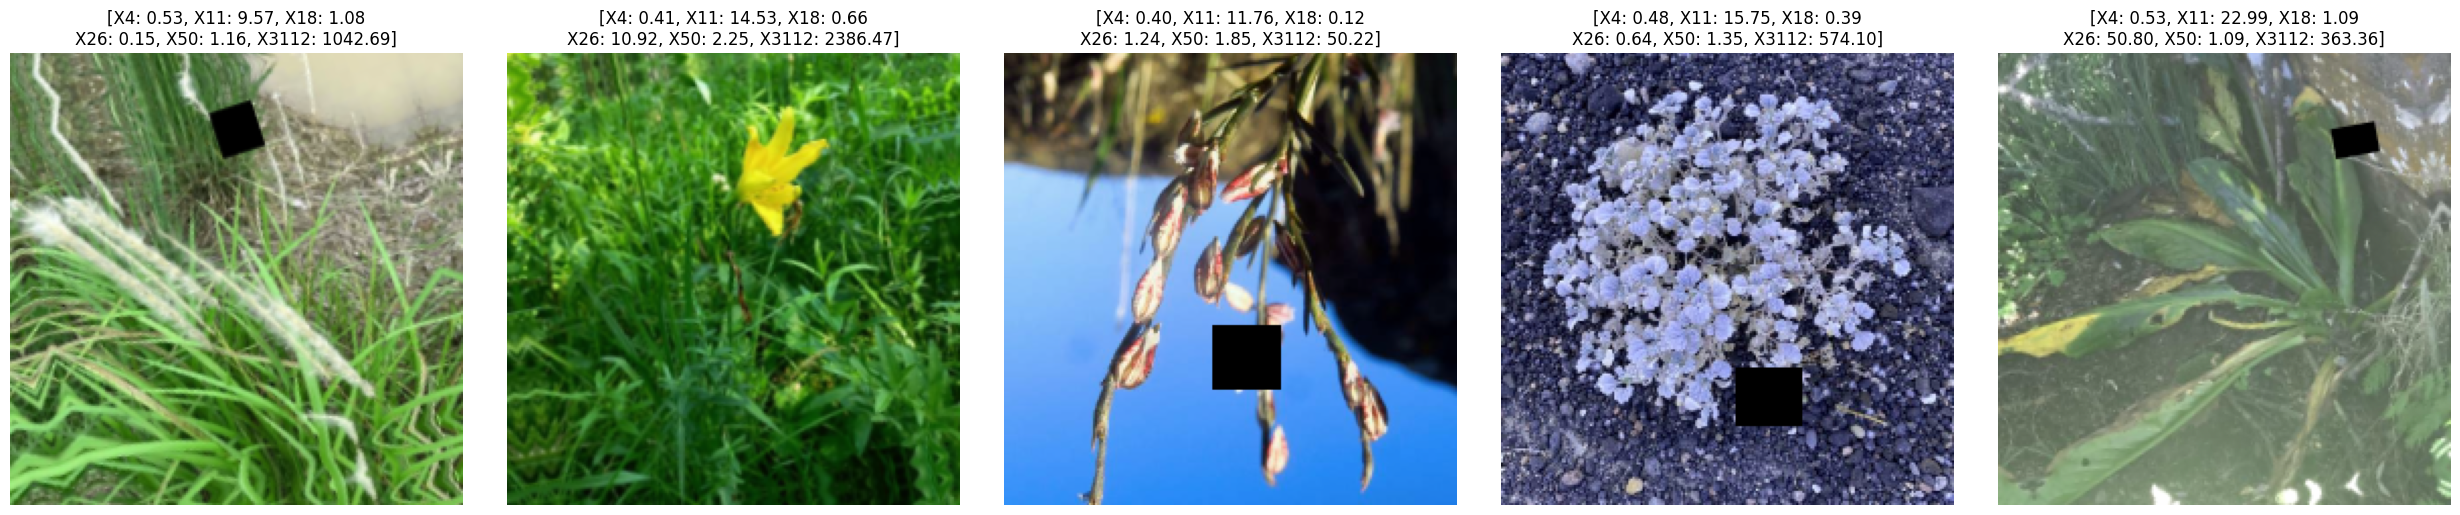
\includegraphics[width=0.9\textwidth]{assets/after_aug_img.png}
    \caption{Random sample of 5 images with augmentations: brightness, rotation, contrast, zoom, hue, cutout, flip, blur, saturation}
\end{figure}

% 5-fold stratified cross-validation + verification and split 
% \cite{Marcot2021} k = 5 good for large sample
% \cite{kequal10isgood} k ~ 10 generally good choice

\smallskip 
In addition to augmentation, we noted that - though not too common - there was still a presence of certain substantial outliers in our data. Through visual inspection, a common reason seems to have been specifically how close an individual was when they took an image. As the training data was labeled by a machine learning model in a supervised fashion, its evident perspective was not something the initial model had learned. As this scaling issue is a byproduct of the initial model, which labeled the data and not any true property of the data, we decided to remove these outliers. We did this by constraining the target distributions to the interval $[0.0001, 0.9999]$ and removing any instances outside of this interval.

\smallskip
Another method of reducing overfitting relevant to apply here is k-fold cross-validation for the data split. We chose $k=5$, as for large datasets, this has proven effective \cite{Marcot2021} and is generally around the commonly chosen value of 10 \cite{kequal10isgood}, where the 0th fold was designated as the validation set. Given that the data is from a geographically large enough sample, we decided to create the folds in a stratified manner under the assumption that the distribution of traits would be reasonably representative of the true distribution and, thus, one the model should learn. This is important as it ensures that the model is trained on a representative sample of the data in each fold and, in turn, has its predictions distributed similarly to the assumed true distribution of the traits. So, we reduce the risk of overfitting to the training data while also ensuring the model is trained using a representative sample of targets in each fold. To validate that the distributions of the target traits are indeed similar, we averaged the distributions of the target traits in each fold, overlayed this on the original distribution of trait means, and normalized them to the same scale.  

\begin{figure}[!h]
    \centering
    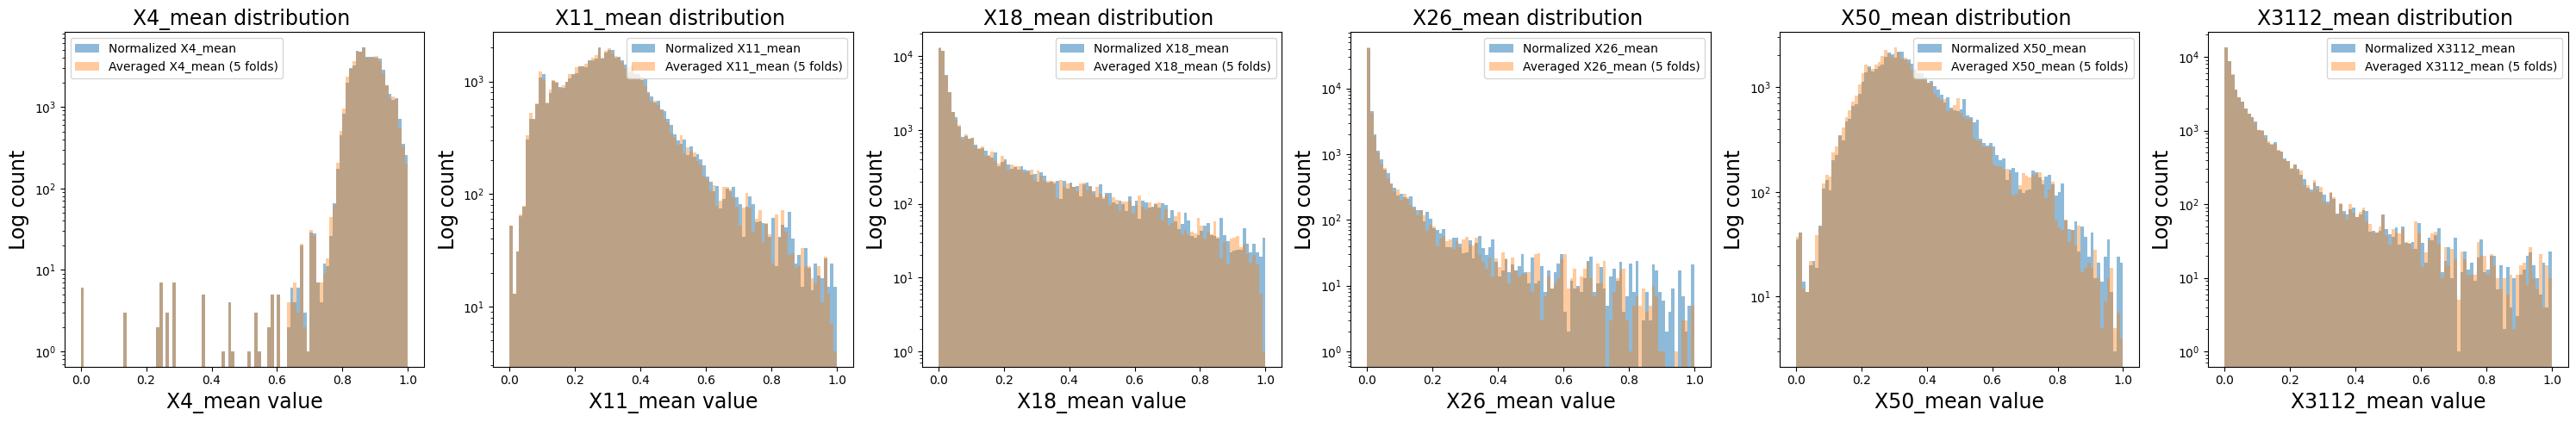
\includegraphics[width=1\textwidth]{assets/distribution_match_folds.png}
    \caption{Comparison of the average trait distributions in each fold with the original distribution of trait means ; (blue) normalized distribution of the trait means across the entire dataset ; (yellow) average normalized distribution of the trait means in each fold}
\end{figure}

\subsection{Model design}

\subsubsection{CNN trained on images}

% give an overview of the model 
    % activation function 
    % batch size
    % optimizer 
    % epochs
Our image CNN is a multi-output model that takes in a tensor consisting of red, green, and blue channels with an image size of 224x224 pixels. The model consists of a trained backbone; in our instance, we compared \textit{efficientnetv2\_b2\_imagenet}, \textit{efficientnetv2\_s\_imagenet}, and \textit{resnet50\_imagenet}. The backbone outputs then feed into a global average pooling layer, followed by two dense layers and a dropout layer connected to the two dense output layers for the main and auxiliary tasks. The hidden layers use a ReLU activation function, and the outputs use no activation function as the targets are continuous. The model is trained using the Adam optimizer with a learning rate of 1e-4, a batch size of 48, and for 12 epochs. Additionally, we used the $R^2$ metric for both loss and evaluation of the model performance, as this is a regression problem. Finally, we used step-based for the learning rate schedule, which was defined as follows:
\[
    \text{lr} = \text{lr}_\text{max} \times d^{\floor*{\frac{e_d}{r}}}
\]
Where $e_d$ is the current epoch, $r$ is the step size (=2), and $d$ is the decay rate.

% talk about the backbones 
    % ResNet 
    % EfficientNet b2 
    % EfficientNet s
\smallskip
Residual Network (ResNet) \cite{he2016identity} introduced in 2016 is a deep learning model that can learn features from images. Most famously, it is known for mitigating the vanishing gradient problem by introducing identity skip connections. We are using \text{ResNet50}, which was trained on imagenet and consists of 48 convolution layers, in addition to a MaxPool and AveragePool layer. EfficientNetV2 \cite{tan2021efficientnetv2} is a family of CNNs from 2021 that have faster speeds than many previous models, primarily by increasing image size during training and incorporating adaptive regularization to compensate for any potential accuracy loss. We are using \textit{efficientnetv2\_b2\_imagenet} and \textit{efficientnetv2\_s\_imagenet}, which are trained on imagenet, with the latter being a smaller (fewer parameters) version of the former. Comparing these backbones in a table, we can get some overview of how they stack up, as seen in \ref{tab:backbone_comparison}

We trained three models with the same architecture but different backbones to compare these backbones. We also specified a contribution of 0.3 to the final loss of the auxiliary task (as opposed to 1.0 for the main task) to limit its impacts on the direction of training. A visual overview of the different models can be seen in \ref{fig:models_overview}. 


\begin{table}[!h]
    \centering
    \begin{tabular}{@{}llll@{}}
    \toprule
    & EfficientNetV2 b2 & EfficientNetV2 s & ResNet50 \\ \midrule
    parameters              & 8.77M             & 20.33M           & 23.56M   \\
    imagenet top 5 accuracy & 94.9\%            & 96.7\%           & (missing)       \\ \bottomrule
\end{tabular}
\caption{Comparison of the different backbones and published top 5 accuracy on imagenet for the specific models}
\label{tab:backbone_comparison}
\end{table}

\begin{figure}[!h]
    \centering
    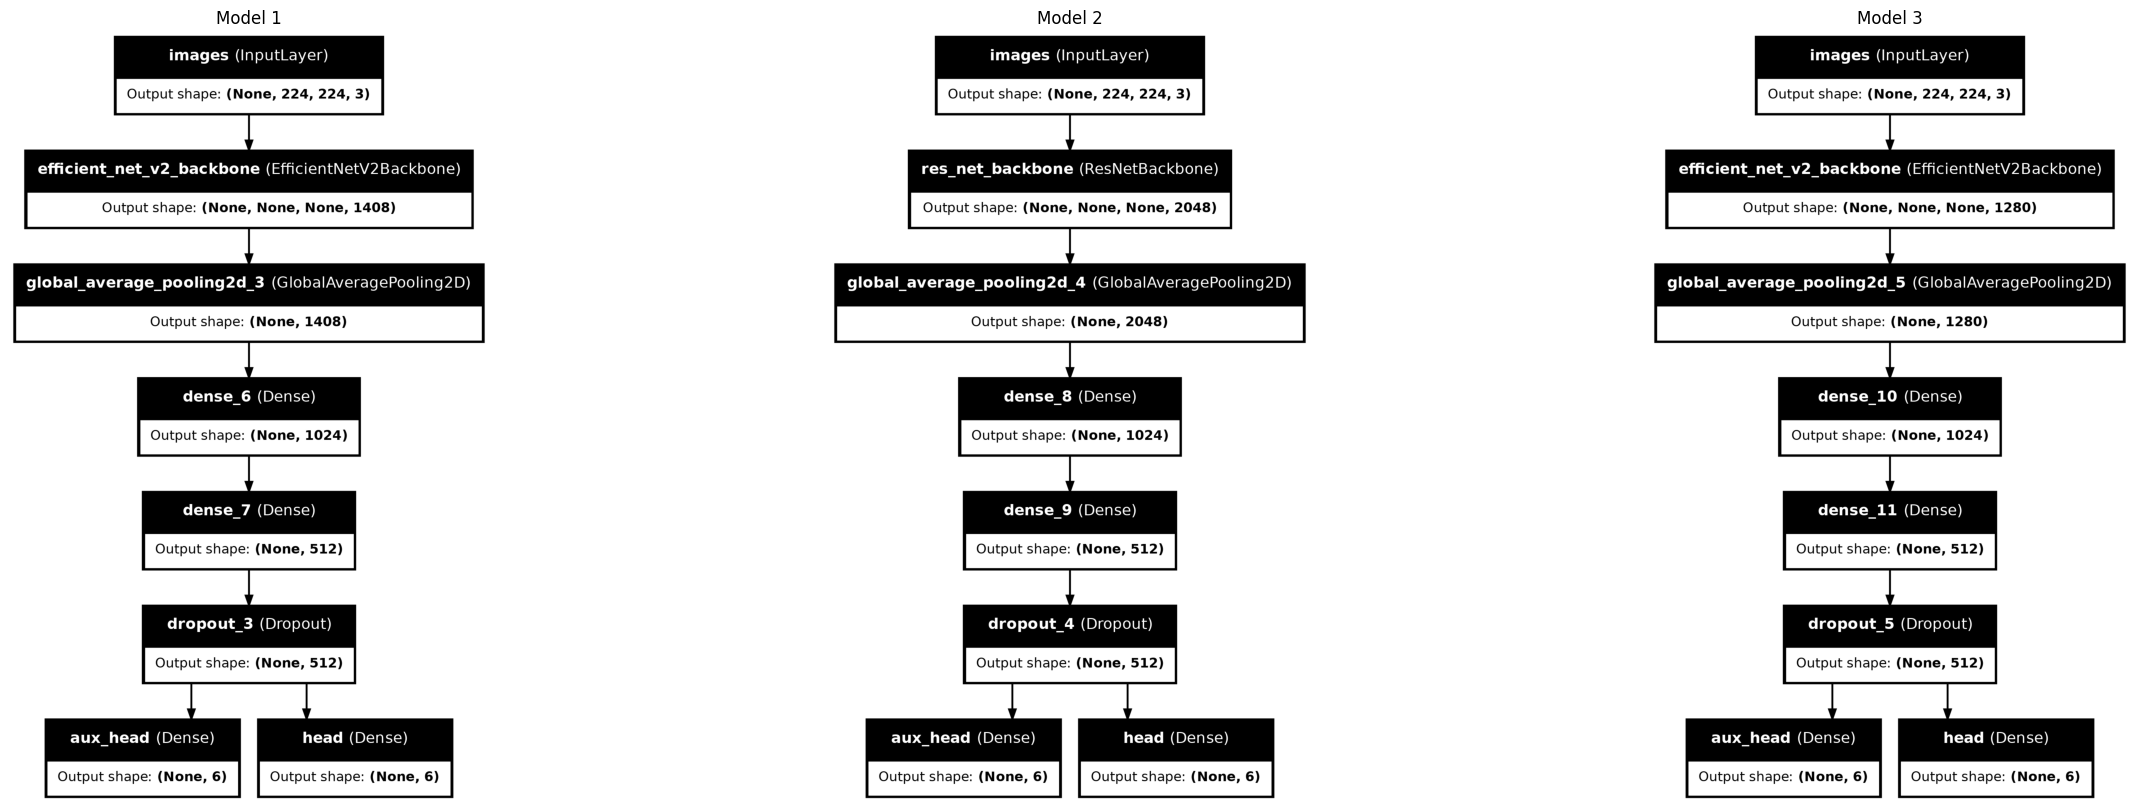
\includegraphics[width=1\textwidth]{assets/different_models.png}
    \caption{Visual overview of the 3 models with different backbones}
    \label{fig:models_overview}
\end{figure}

\subsubsection{Image CNN tuning}

% model x had the best loss in the end 
Looking at the results in \ref{fig:different_backbones} of the initial choice of hyperparameters for the different models, we first noticed similar behavior of all the $R^2$ values in terms of their sign. The coefficient of determination is defined as follows:

\[
    R^2 = 1 - \frac{\sum_{i=1}^{n} (y_i - \hat{y}_i)^2}{\sum_{i=1}^{n} (y_i - \bar{y})^2} = 1 - \frac{SS_{res}}{SS_{tot}}  
\]
Where $SS_{res}$ is the residual sum of squares and $SS_{tot}$ is the total sum of squares. One observation in our results was that for all instances, we had a negative $R^2$, implying that $SS_{res} > SS_{tot}$ meaning our model performs worse than the baseline at $SS_{res} = SS_{tot}$. This is a clear indication that the model is fitting against the data. Numerous reasons could be the cause of this. Due to the results of the initial training not being conclusive in regards to which model is better, we decided to simply continue with the model using the \textit{efficientnetv2\_b2\_imagenet} backbone as it has a high top 5 accuracy while also having fewer parameters.

\begin{figure}[!h]
    \centering
    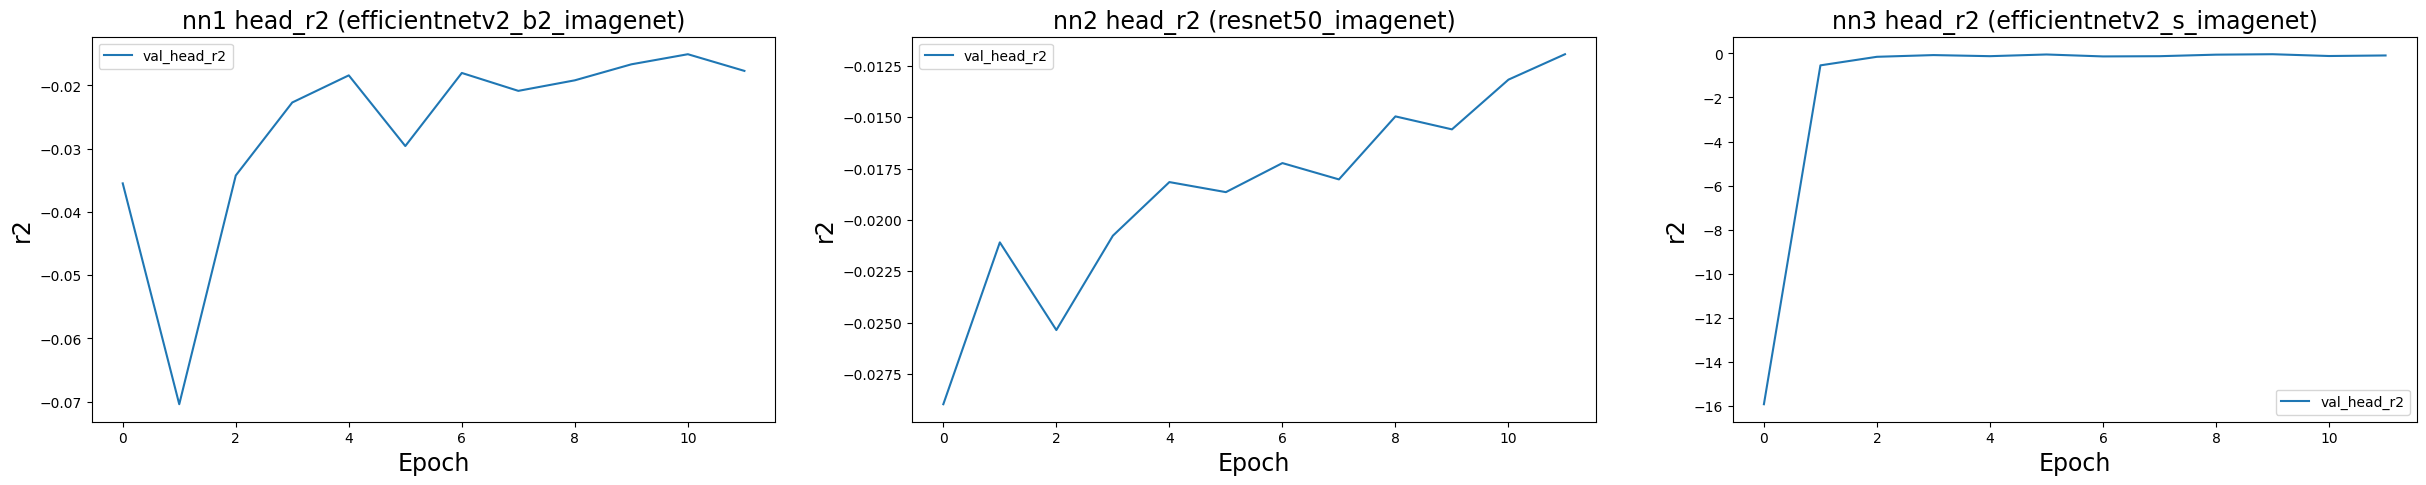
\includegraphics[width=1\textwidth]{assets/different_backbones.png}
    \caption{Validation $R^2$ for primary task with different backbones}
    \label{fig:different_backbones}
\end{figure}

Both of the EfficientNet backbones exhibit similar behavior as they come from the same family of models; this being a fast convergence, though also an early plateau at a more suboptimal loss. The ResNet50 backbone, on the other hand, has a slower convergence but a more consistent decrease in loss (increase in $R^2$). This could indicate that the ResNet50 backbone has a greater potential to learn from the data, albeit in a slower manner. 

\smallskip 
The learning rate schedule was one of the first things we decided to test. We tested three schedules: step-based (baseline), exponential, and cosine annealing. The results demonstrated in \ref{fig:lr_schedules} show that the cosine annealing and exponential schedule had a slower convergence than the step-based schedule and a more erratic behavior.  

\begin{figure}[!h]
    \centering
    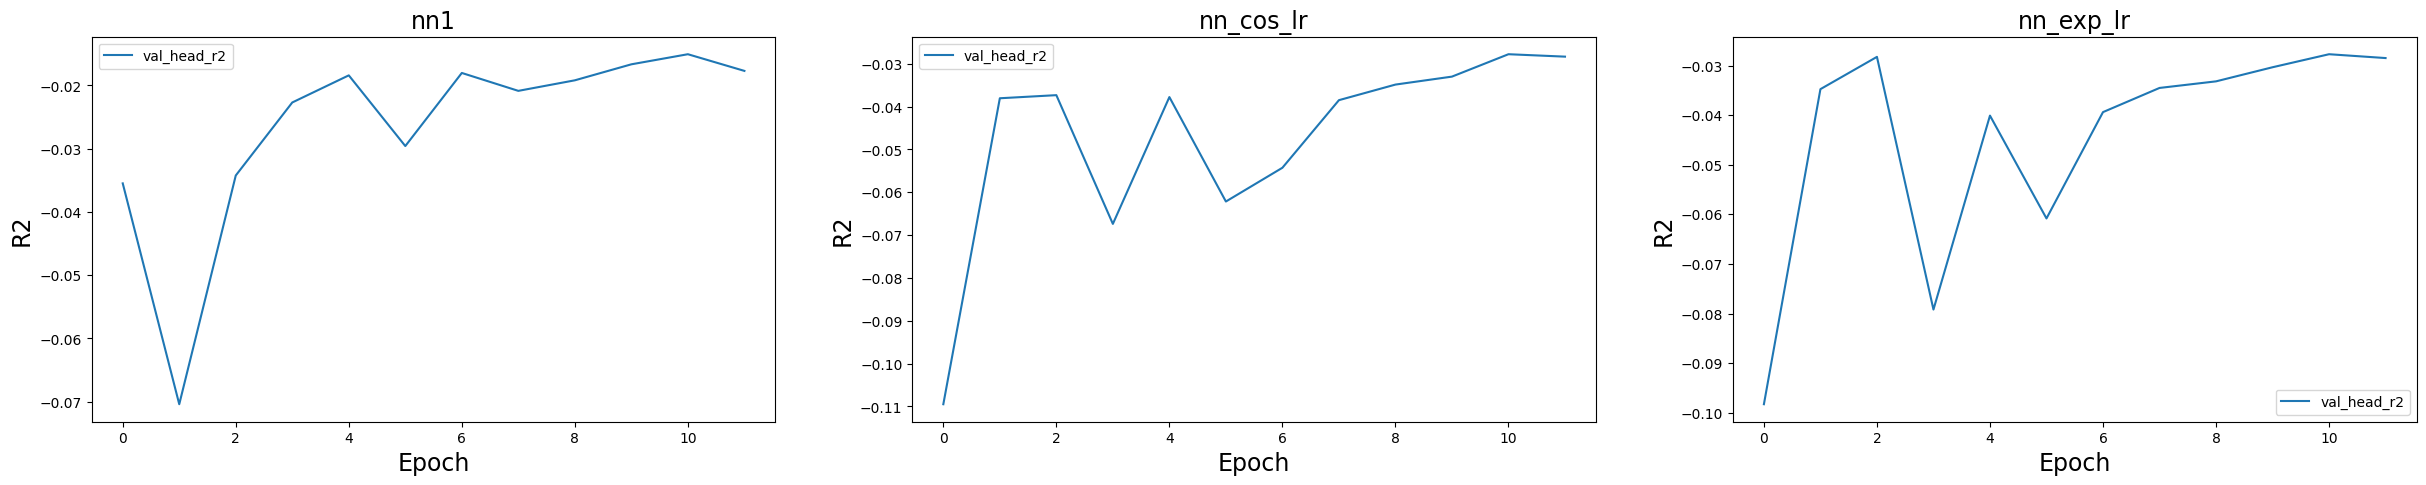
\includegraphics[width=1\textwidth]{assets/lr_schedule_diffs.png}
    \caption{Comparison of different learning rate schedules ; (left) step-based ; (center) cosine annealing ; (right) exponential}
    \label{fig:lr_schedules}
\end{figure}

% we wanted to test out : different lr, backbone training on vs off 
    % test out cosine annealing 
    % test out exp 
    % plot step vs exp vs cosine annealing

Another point of consideration we had was the training of the backbone. We wanted to test whether there was any difference in $R^2$ when we allowed the model to adapt the weights of the backbone. These results can be seen in \ref{fig:backbone_training}. In both instances, we see the model converging at around the second epoch and hitting a plateau of $\approx -0.03 R^2$. This is likely due to the fact that the backbone requires little additional training to learn the features from the data and generalizes well to this task.

    % test out backbone training off for best lr schedule 
    % test out backbone training on for best lr schedule

\begin{figure}[!h]
    \centering
    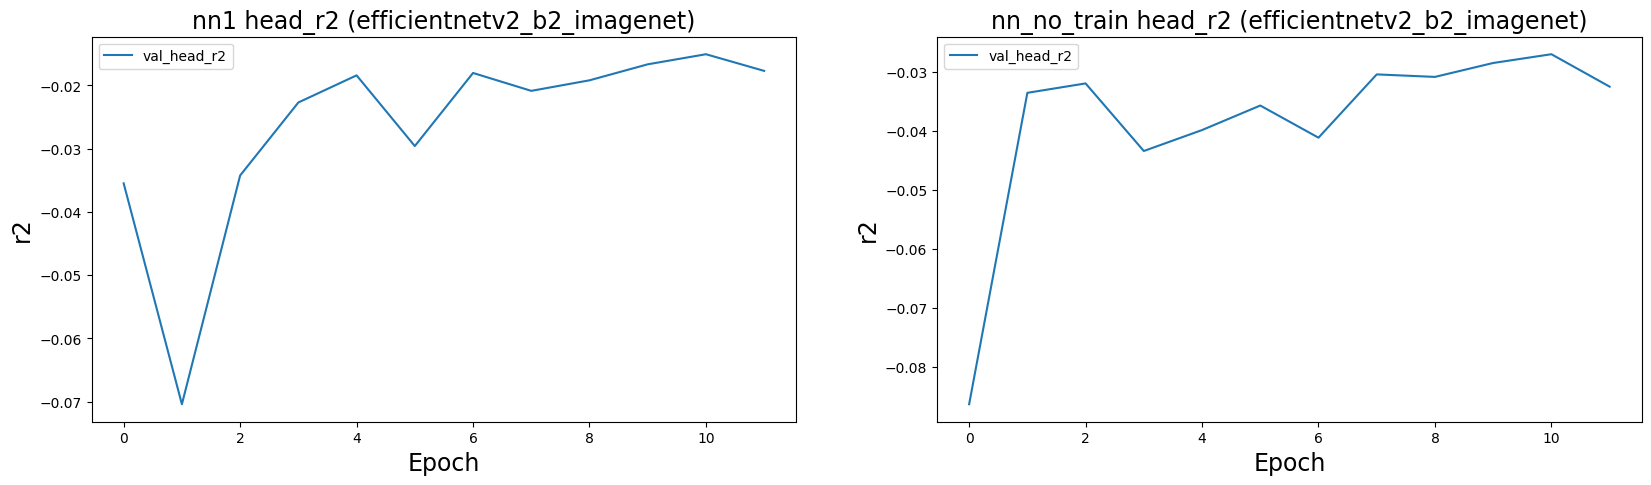
\includegraphics[width=0.7\textwidth]{assets/train_vs_notrain.png}
    \caption{Comparison of models with backbone training on (right) and off (left)}
    \label{fig:backbone_training}
\end{figure}

\subsubsection{CNN trained on images and geodata}

To construct the CNN trained on images and geodata, we first created the two branches of the model, one to take in the image data and reduce it to a 1-tensor and, similarly, one to extract features from the tabular data. The two branches were then concatenated and fed to the main and auxiliary task dense output layers. As the only difference here is the additional branch for the geodata, we kept the hyperparameters the same to get a fair comparison between both approaches. A visual overview of the model can be seen in \ref{fig:geodata_model}.

\begin{figure}[!h]
    \centering 
    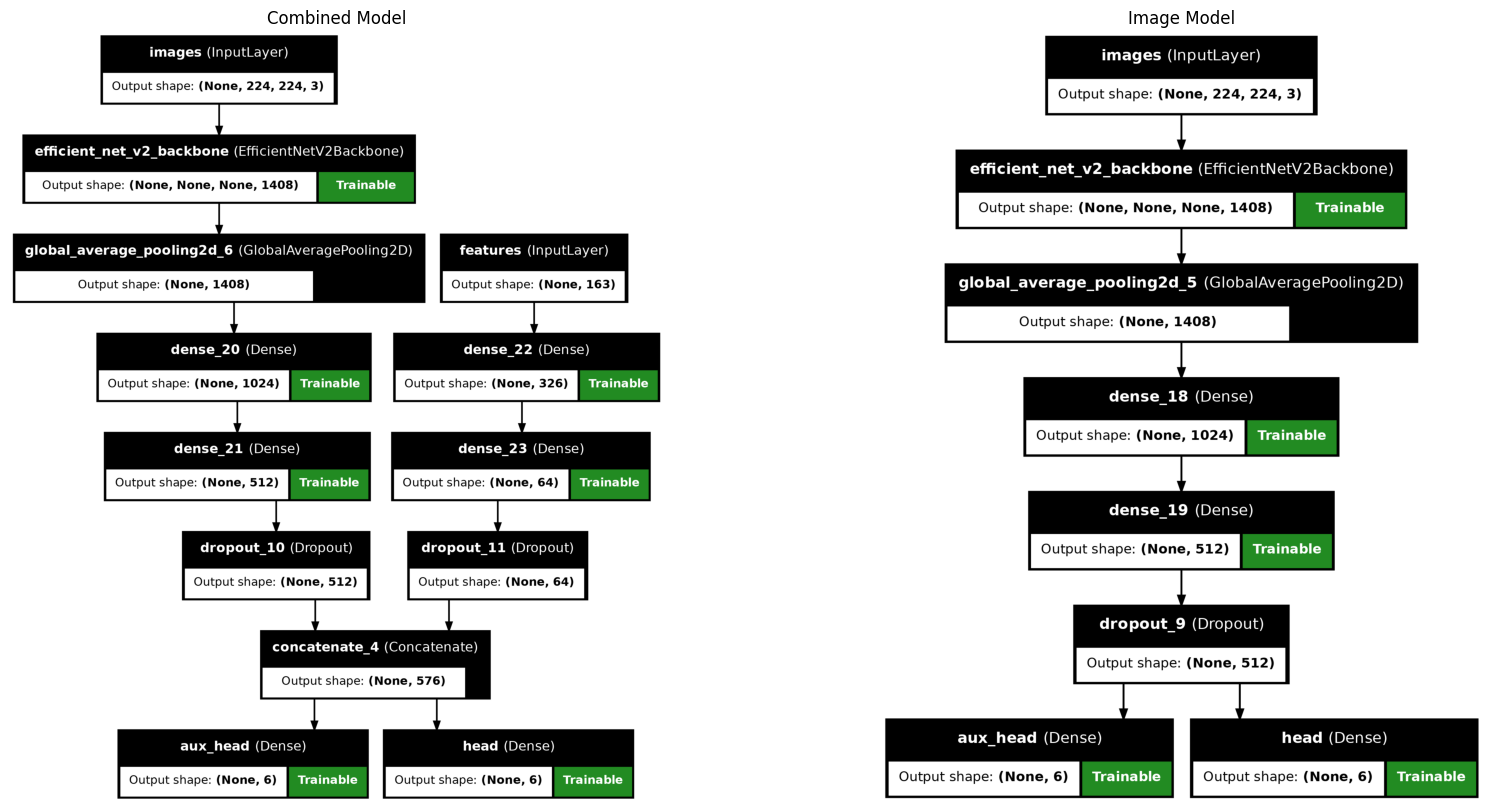
\includegraphics[width=0.8\textwidth]{assets/img_geo_model.png}
    \caption{(right) Model architecture of the CNN trained on images and geodata; (left) Model architecture of the CNN trained on images alone}
    \label{fig:geodata_model}
\end{figure}

% give an overview of the model
    % mention mainly the geodata model 
    % show a plot of the model

\subsection{Model comparative evaluation}

% evaluation of individual models 

For the final comparison, we first looked at the basic evaluation metrics of either model. These results can be seen in \ref{fig:basic_evaluation}. We can see that the model trained on images and geodata has a lower $R^2$ than the model just trained on images, though not by any significant margin. 

\begin{figure}[!h]
    \centering
    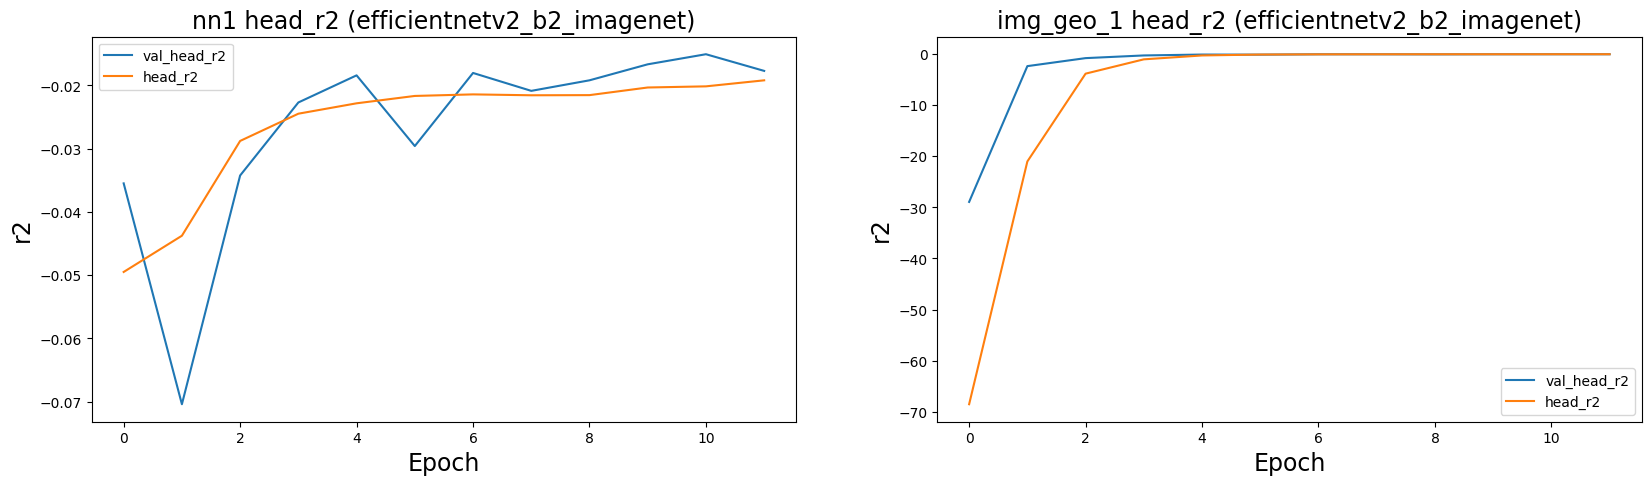
\includegraphics[width=0.8\textwidth]{assets/fin_img_vs_geo.png}
    \caption{Basic evaluation metrics of the two models}
    \label{fig:basic_evaluation}
\end{figure}

% comparative evaluation
\begin{table}[!h]
    \centering
    \begin{tabular}{@{}llll@{}}
    \toprule
    & Image model & Combined model \\ \midrule
    test set $R^2$              & -6.18163             & -381.62190   \\ \bottomrule
\end{tabular}
\caption{Comparison of the $R^2$ on the test set for the two models}
\end{table}

\section{Results}

Even though the $R^2$ did not vary by a significant margin between the combined and image model, the $R^2$ on the test set did. While both models still had a negative $R^2$ for the test set, the image model had a higher $R^2$ than the combined model. One potential explanation is that the model is overfitting on some property derived from the training data. The source of this issue would then reasonably lie with the inclusion of the geodata. While, in theory, the geodata does provide more context to the model and thus should give it a greater potential to learn from the data, it could also be the case that the model is learning from the geodata in a way that is not beneficial to the prediction of the plant traits.   

\section{Discussion}

% discuss the results
Predicting plant traits from images and geodata is a complex task requiring a CNN to learn and extract features from images and geodata. The results of our work show that a CNN trained on just an image outperforms one trained on images and geodata. Neither of the models elaborated here is necessarily a good predictor; one of the main reasons for this is likely the complexity and nuance of the regression task. We now propose various directions for future work to improve the models' prediction capabilities.

Hyperparameter tuning is one of the most important aspects of training a machine learning model. In our work, we only tested a few different learning rate schedules and backbones using a greedy optimization approach. Random search - which has been demonstrated to be more effective than grid search \cite{JMLR:v13:bergstra12a} - would likely have been a better choice, albeit more computationally expensive. In addition, we predominantly looked at hyperparameters, but varying the model architecture could have also been a beneficial direction. A larger model could learn more nuanced features in the data. 

The training data itself can also be modified to improve the model. Certain plant traits rely on some sense of relative scale to be elicited accurately (e.g., we know that a tree is bigger than a flower regardless of image angle). However, this scale is easily lost due to the variability in how people take photos. One way of mitigating this could be to incorporate scale normalization through Depth Estimation; previous work \cite{Ummenhofer_2017} demonstrated the ability to train CNNs on the DIODE (Dense Indoor/Outdoor DEpth) \cite{vasiljevic2019diode} dataset to estimate depth. The images' learned depth information could then be used as a moderator to scale the images to a common scale, possibly improving the prediction capabilities.

How adaptable pre-trained models are to new tasks could also be further explored. Kunze et al. \cite{kunze2017transfer} answered this question by looking at the weight difference distribution per layer early and late into training. They found that models trained on a similar task to the target domain only had a minor change in the weight distribution. This reasoning could be applied to more accurately find the optimal backbone. Additionally, the use of a pre-trained model could be further explored by looking at the effect of the number of layers frozen during training. 

\newpage
\section{Conclusion}

This paper aimed to evaluate the effectiveness of incorporating ancillary geodata alongside images in a Convolutional Neural Network (CNN) for predicting plant traits from images. Our key findings revealed that integrating both data types into models resulted in faster convergence, but it did not improve the predictive accuracy of models trained solely on images. This result indicates that adding geodata does not necessarily translate into better performance, and it highlights the complexity of the task at hand.

We faced several challenges during our research, such as the negative R² values of the models, which suggest underfitting or other core limitations in our models. Additionally, varying image quality and the presence of outliers complicated model training and performance, highlighting the importance of data quality and preprocessing for developing effective predictive models. 

For future work, we suggest exploring alternative hyperparameters, diverse model architectures, and better data augmentation techniques. Incorporating depth estimation for scale normalization could be a promising method for addressing the variability present in image-based data. Investigating the adaptability of pre-trained models to this specific domain could also provide valuable insights into optimizing model training and performance.

Our research highlights the potential of machine learning in ecological research, specifically in understanding and responding to the impact of climate change on plant life. Despite the challenges, continued innovation and exploration can uncover deeper insights into the planet's biological responses to a changing climate, which is crucial for global conservation and sustainability efforts.

\printbibliography


\title{MLVU information sheet}
\author{}
\date{}
\maketitle

\noindent \textit{Please include this page in your report either at the start or at the end, before the appendix. Do not change the formatting.}

\paragraph{Group number}~

02

\paragraph{Authors}~

\begin{tabular}{r r}
name &student number \\
\hline
Kai Niermann & 2720905 \\
Dávid Miklo & 2767001 \\
Trix Taiclet & 2785891 \\
Conner Dassen & 2695049 \\
Red Kaláb & 2735630 \\
\end{tabular}

\paragraph{Software used} \textit{jupyter, python3.10, keras3, tf2.16, various data viz libraries, gcp compute engine to train the models, pandas for most of the data science related tasks}

\paragraph{Use of AI tools} \textit{}
\paragraph{Link to code (optional)} \textit{}

\paragraph{Group disagreements} \textit{}

\end{document}

